% \part{Equipment Tour}

\chapter{Overview}
\label{sec:eq_intro}

\section{Introduction}
\label{sec:eq_intro:intro}

The University of Virginia is part of the CMS experiment at CERN.  The CMS detector is a multistage general purpose detector.  The first inner stage of the detector is the electromagnetic calorimeter (Ecal).  The central cavity of CMS is cylindrical, with the beam coming in along its axis.  The walls of the cylinder are formed by the Ecal detectors.  The rounded walls are the barrel, and at either end are the endcaps.  The detectors are made of two main components.  The masses that react with the beam products are dense inorganic PbWO$_4$ (\textit{``lead-tungsten-tetroxide''}) scintillator crystals.  Behind those scintillators are the scintillation detectors.  In the barrel, these detectors are avalanche photodiodes (AVDs.)  In the endcap, these detectors are Vacuum Photo-Triodes (VPTs.)

\begin{figure}[htbp]
  \centering
  \parbox{0.75\textwidth}{\tiny
    Taken from K.W. Bell et al., ``\href{papers/1344324}{Vacuum Phototriodes for the CMS Electromagnetic Calorimeter Endcap},'' IEEE Transactions on Nuclear Science, vol. 51, no. 5, pp. 2284-2287, 2004.}
  \pgfimage[interpolate=true]{figures/ecal_cutaway}
  \caption{Schematic View of CMS Electromagnetic Calorimeter}
  \label{fig:eq_intro:ecal}
\end{figure}

As the beam comes in on-axis, the majority of the beam products are produced just off-axis.  This means that the endcaps receive the highest radiation dosage, and the detectors need to be especially hardened against neutron radiation.  The PbWO$_4$ crystals scintillate in the visible spectrum, near 420\,nm.   The faceplates of the VPTs are made of a radiation-hard UV-transmitting borosilicate glass.  Glass tends to darken when exposed to neutron radiation.  The glass used for the VPT faceplates is manufactured in small batches and is proven to have less than 10\,\% transmission loss after a dose of 20\,kGy over a 48\,hour period using a $^{60}$Co source, prior to being accepted for use in VPT production.

The exact performance characteristics of VPTs under extended optical loads in strong magnetic fields are still being studied.  The University of Virginia has previously studied their performance under temperature variation, and also under a non-axial magnetic field (\secnameref{chap:previous}.)  We are currently (Summer 2010) studying their long term response behavior, which has been shown to decay over time.

\section{Experimental Setup \textcolor{red}{[DRAFT]}}
\label{sec:eq_intro:setup}

The experimental setup at UVa has two main sections: The \Gls{PXI Crate} and the \Gls{rig}.  The \gls{PXI Crate} sends signals from its \pxislottwo{}~\gls{FPGA} module to the rig's \glspl{LED board}.  The boards send a photon pulse to VPTs housed inside a 3.8\,T magnetic field, and the VPT translates those photons into a charge on its anode.  The anode signal is amplified by a Stephenson amplifier, and that amplified signal is sent back to the PXI Crate's \pxislotn{3}~Switch.  The PXI Crate then processes and records the signals.

Conceptually part of the rig, a high voltage supply provides a +800\,V and +600\,V potential difference to the VPT's anode and dynode, respectively.  A low voltage supply provides power to the LED pulser boards and the Stephenson amplifier.

\begin{figure}[htbp]
  \centering
  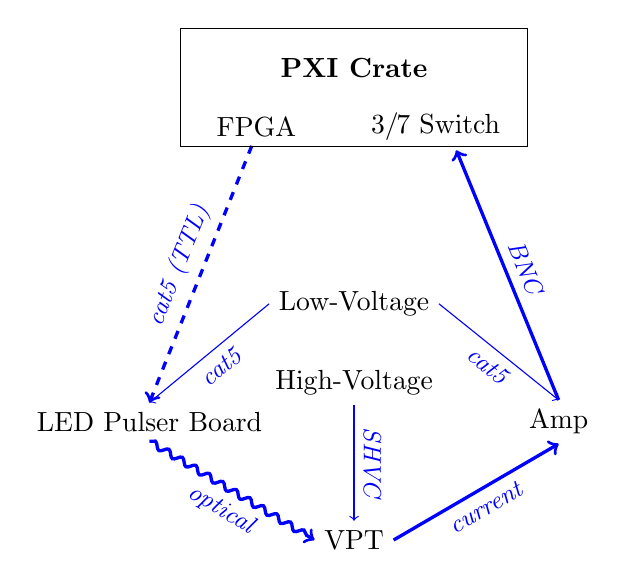
\begin{tikzpicture}
    
    \node (vpt) at (0,0) {VPT};
    \node (led) at (150:3) {LED Pulser Board};
    \node (amp) at (30:3) {Amp};
    \node (hv)  at (90:2) {High-Voltage};
    \node (lv)  at (90:3) {Low-Voltage};
    \node (pxi) at (90:6) {\bfseries PXI Crate};
    \path (pxi) node (switch) at +(-30:1.5) {\hspace{-1.5em}\pxislotn{3}/\hspace{-.2ex}\pxislotn{7}\ Switch};
    \path (pxi) node (fpga)   at +(210:1.5) {\pxislottwo\ FPGA};

    \begin{scope}[blue]
    \path[->] (fpga.south) edge[dashed,very thick]
                                        node[above,sloped] {\itshape\small cat5 (TTL)}      (led.north);
    \path[->] (led.south)  edge[very thick,decorate,decoration={snake,amplitude=.4mm,segment length=2mm,post length=1mm}]
                                        node[below,sloped] {\itshape\small  optical} (vpt.west);
    \path[->] (vpt.east)   edge[solid,very thick]
                                       node[below,sloped] {\itshape\small  current} (amp.south);
    \path[->] (amp.north)  edge[solid,very thick]
                                        node[above,sloped] {\itshape\small  BNC}     (switch.south);
    \path[->] (lv.west)    edge[thin]   node[below,sloped] {\itshape\small  cat5}    (led.north);
    \path[->] (lv.east)    edge[thin]   node[below,sloped] {\itshape\small  cat5}    (amp.north);
    \path[->] (hv.south)   edge[thin]   node[above,sloped] {\itshape\small  SHVC}    (vpt.north);
    \end{scope}

    \draw (pxi) ++(-90:1) ++(left:2.2) rectangle ++(4.4,1.5);
    
  \end{tikzpicture}
  \caption{Rig Connections}
  \label{fig:eq_intro:rig_connections}
\end{figure}

\subsection{LED Branch}
\label{sec:eq_intro:led_branch}

The FPGA sends three TTL signals to the powered LED board, which each correspond to a single LED (\seeref{sec:eq_led}.)

\FIXME\ Fix the list style, and Fix the sentence structure: eg, ``The Load signal is...''

\begin{description}
\item [1. Load] A simple simulated collider beam signal, intended to represent photon activity during beam events.
\item [2. Soak] A faux load between beam events to maintain the VPT's response curve.
\item [3. Reference] A measurement pulse is inserted between the load and soak pulses to measure the VPT's response characteristics.
\end{description}

Each of the three optical signals that the LED board emits are multiplexed into six different fiber optic cables.  One of each of those fibers connects to a factory-callibrated PIN diode.  The PIN diode's signal can be used to make adjustments due to variations in LED light output.  The remaining five fibers terminate in light-sealed boxes containing one VPT each, and project their light onto the VPT's photocathode.  So, in total, each VPT receives three fibers (one from each LED), and there are three PIN diodes acting as references for LED light output.

\begin{figure}[htbp]
  \centering
  \begin{tikzpicture}[scale=0.75]
  \begin{scope}[xshift=10cm]
    %%%% North Endcap %%%%%%%%%%%%%%%%%%%%%%%%%%%%%%%%%%%%%%%%%%%%%%%%%%%%
    \begin{scope}[yscale=-1,fill=white]
      \draw[black,xscale=0.3,yscale=0.25,yshift=-7.1cm,fill=white]
           (-2,-1.2) coordinate (a)
        -- coordinate (ab) (-2,0) coordinate (b)   
        .. coordinate (bc) controls (-2,0.2) and (2,0.2) .. (2,0) coordinate (c)
        -- (2,-1.2) coordinate (d)
        .. coordinate (de) controls (2,-1.4) and (-2,-1.4) .. (-2,-1.2) coordinate (e);
      \draw[black,xscale=0.91,yscale=0.91,yshift=-.18cm,fill=white]
           (-2,-1.2) coordinate (sea)
        .. coordinate (ad) controls (-2,-1.0) and (2,-1.0) .. (2,-1.2)
        .. coordinate (de) controls (2,-2.15) and (-2,-2.15) .. (-2,-1.2) coordinate (-2,-1.2);
    \end{scope}

    %%%% Barrel %%%%%%%%%%%%%%%%%%%%%%%%%%%%%%%%%%%%%%%%%%%%%%%%%%%%%%%%%%
    \draw[black,fill=white]
          (-2,-1.2) coordinate (a)
       -- coordinate (ab) (-2,1.2) coordinate (b) 
       .. coordinate (bc) controls (-2,1.4) and (2,1.4) .. (2,1.2) coordinate (c)
       -- (2,-1.2) coordinate (d)
       .. coordinate (de) controls (2,-1.4) and (-2,-1.4) .. (-2,-1.2) coordinate (e)
       .. coordinate (ad) controls (-2,-1.0) and (2,-1.0) .. (d);

    \draw[black,fill=white]
         (-2.11,-.13)
      -- ++(0,.2)
      .. controls (-2,.36) and (2,.36) .. (2.11,.07)
      -- ++(0,-.2);

    \draw[black,fill=white]
         (-2,-.2)
      .. controls (-2,0) and (2,0) .. ( 2,-.2)
      .. controls (3,.08) and (-3,.08) .. (-2,-.2) --cycle;

    %%%% South Endcap %%%%%%%%%%%%%%%%%%%%%%%%%%%%%%%%%%%%%%%%%%%%%%%%%%%%
    \begin{scope}
    \draw[xscale=0.91,yscale=0.91,yshift=-.18cm,fill=white]
         (-2,-1.2) coordinate (sea)
      .. coordinate (ad) controls (-2,-1.0) and (2,-1.0) .. (2,-1.2)
      .. coordinate (de) controls (2,-2.15) and (-2,-2.15) .. (-2,-1.2) coordinate (-2,-1.2);
    \draw[xscale=0.3,yscale=0.25,yshift=-7.1cm,fill=white]
         (-2,-1.2) coordinate (a)
      -- coordinate (ab) (-2,0) coordinate (b) 
      .. coordinate (bc) controls (-2,0.2) and (2,0.2) .. (2,0) coordinate (c)
      -- (2,-1.2) coordinate (d)
      .. coordinate (de) controls (2,-1.4) and (-2,-1.4) .. (-2,-1.2) coordinate (e)
      .. coordinate (ad) controls (-2,-1.0) and (2,-1.0) .. (d);
    \end{scope}
  \end{scope}

  \node at (1,0) {\bfseries PXI Crate};
  \begin{scope}[xshift=1cm]
    \node[chamfered rectangle, white, fill=blue, double=blue, draw, very thick]
    (FPGA) at (0,-1) {\bfseries FPGA};
    \node[chamfered rectangle, white, fill=blue, double=blue, draw, very thick]
    (Switch) at (0,1) {\bfseries Switch};
  \end{scope}

  \draw[very thick]
         (FPGA)
      -- ++(down:2cm) coordinate (aa);
  \draw[very thick]
         (10,-3) coordinate (bb)
      -- ++(up:1cm-.05cm);

  \draw (aa) -- (bb)
    -- ++(up:.2) -- ++(left:9)
    -- ++(up:.2) -- ++(right:9);

  \node[] at (10-4.5-1.5 ,-2.5)  {\tiny\scshape load};
  \node[] at (10-4.5     ,-2.7)  {\tiny\scshape soak};
  \node[] at (10-4.5+1.5 ,-2.9)  {\tiny\scshape reference};

  \draw[very thick]
       (Switch)
    -- ++(up:2) coordinate (cc);
  \draw[very thick]
       (10,3) coordinate (dd)
    -- ++(down:1-.1);
  \draw (cc) -- (dd)
    -- ++(down:.2) -- ++(left:9)
    -- ++(down:.2) -- ++(right:9)
    -- ++(down:.2) -- ++(left:9)
    ;%-- ++(down:.2) -- ++(right:9);
 

  \node[] at (10-4.5-1.5 ,3.1) {\tiny\scshape anode};
  \node[] at (10-4.5     ,2.9) {\tiny\scshape cathode};
  \node[] at (10-4.5+1.5 ,2.7) {\tiny\scshape pin diode};
  \node[] at (10-4.5-1.5 ,2.5) {\tiny\scshape humiter};
  \node[] at (10-4.5-1.5 ,2.3) {\tiny\scshape };
\end{tikzpicture}

  \caption{Signal Path in Teststand}
  \label{fig:eq_intro:signal}
\end{figure}


\subsection{VPT Branch}
\label{sec:eq_intro:vpt_branch}
A VPT (\secnameref{sec:eq_vpt}) is a single stage photomultiplier.  The VPT's photocathode, dynode, and anode accumulate charge as light impacts the photocathode, with the most charge accumulating on the anode.  As photons  strike the photocathode, electrons are liberated.  A large potential of $+600$\,V is driven from the photocathode to the dynode,   The current from the VPT's anode and cathode are ultimately routed to the PXI Crate's switches, and then on to the crate's DMM or oscilloscope.  Before that, they go through an amplification stage.

The VPT's anode is connected directly to a Stephenson amplifier (\secnameref{sec:eq_preamp}), which connects to the \pxislotn{7} high-frequency switch.  The PIN diode signal passes unmodified to that same \pxislotn{7} high-frequency switch.  The VPT's cathode signal passes through a \FIXME 100x powered amplifier before connecting to the \pxislotn{3} low-frequency switch.

A temperature and humidity monitor is mounted next to the rig, connected to the \pxislotn{3} low-frequency switch.


%%% Local Variables: 
%%% mode: latex
%%% TeX-master: "Manual"
%%% End: 
